\documentclass{labreport}

\usepackage[T1]{fontenc}
\usepackage[utf8]{inputenc}
\usepackage{lmodern}
\usepackage{microtype}
\usepackage{booktabs}
\usepackage{hyperref}
\usepackage{listings}
\usepackage{xcolor}
\usepackage{float}
\usepackage{colortbl}
\usepackage{amsmath}
\usepackage{graphicx}
\usepackage{minted}

% Konfiguracja kolorowania składni dla Python
\setminted[python]{
    linenos,
    bgcolor=gray!10,
    fontsize=\small,
    breaklines
}

% Ustawienie środowiska dla konsoli (terminala)
\newminted[console]{text}{
    bgcolor=black,
    fontfamily=tt,
    fontsize=\small,
    formatcom=\color{white},
    breaklines
}

\reporttitle{Raport z~etapu 11}{Przetwarzanie dużych zbiorów danych}
\author{
    Szymon Jędrzejczak (266867) \\
    Mateusz Nasewicz (268513) \\
    Szymon Wieczorek (266586) \\
}
\date{08.06.2026}

\begin{document}

\maketitle
\tableofcontents
\newpage

% ============================================================
\section{Konfiguracja środowiska chmurowego}
% ============================================================

Potok przetwarzania danych przeniesiono na platformę \textbf{Databricks Free Edition} z~wykorzystaniem obliczeń serverless (Serverless Compute, środowisko \texttt{client=2}). Infrastruktura zarządzana jest przez \textbf{Terraform} -- definicje jobów, Unity Catalog oraz pliki źródłowe wgrywane są automatycznie przy każdym \texttt{terraform apply}.

\subsection{Unity Catalog -- przechowywanie danych}

Dane wejściowe i~wyniki pośrednie przechowywane są w~\textbf{Unity Catalog Volume} pod ścieżką \texttt{/Volumes/workspace/duze\_dane/data/}. Schemat \texttt{duze\_dane} i~wolumen \texttt{data} tworzone są przez Terraform. Rysunek~\ref{fig:catalog} przedstawia zawartość wolumenu po wykonaniu pełnego potoku -- widoczne są katalogi z~danymi wejściowymi (\texttt{gtfs}, \texttt{osm\_csv}, \texttt{real\_estate\_geocoded}) oraz wynikami wszystkich etapów (\texttt{t1\_1}, \texttt{t1\_2}, \texttt{t1\_3}, \texttt{t1\_5}, \texttt{t2}, \texttt{t3}) i~eksperymentów.

\begin{figure}[H]
    \centering
    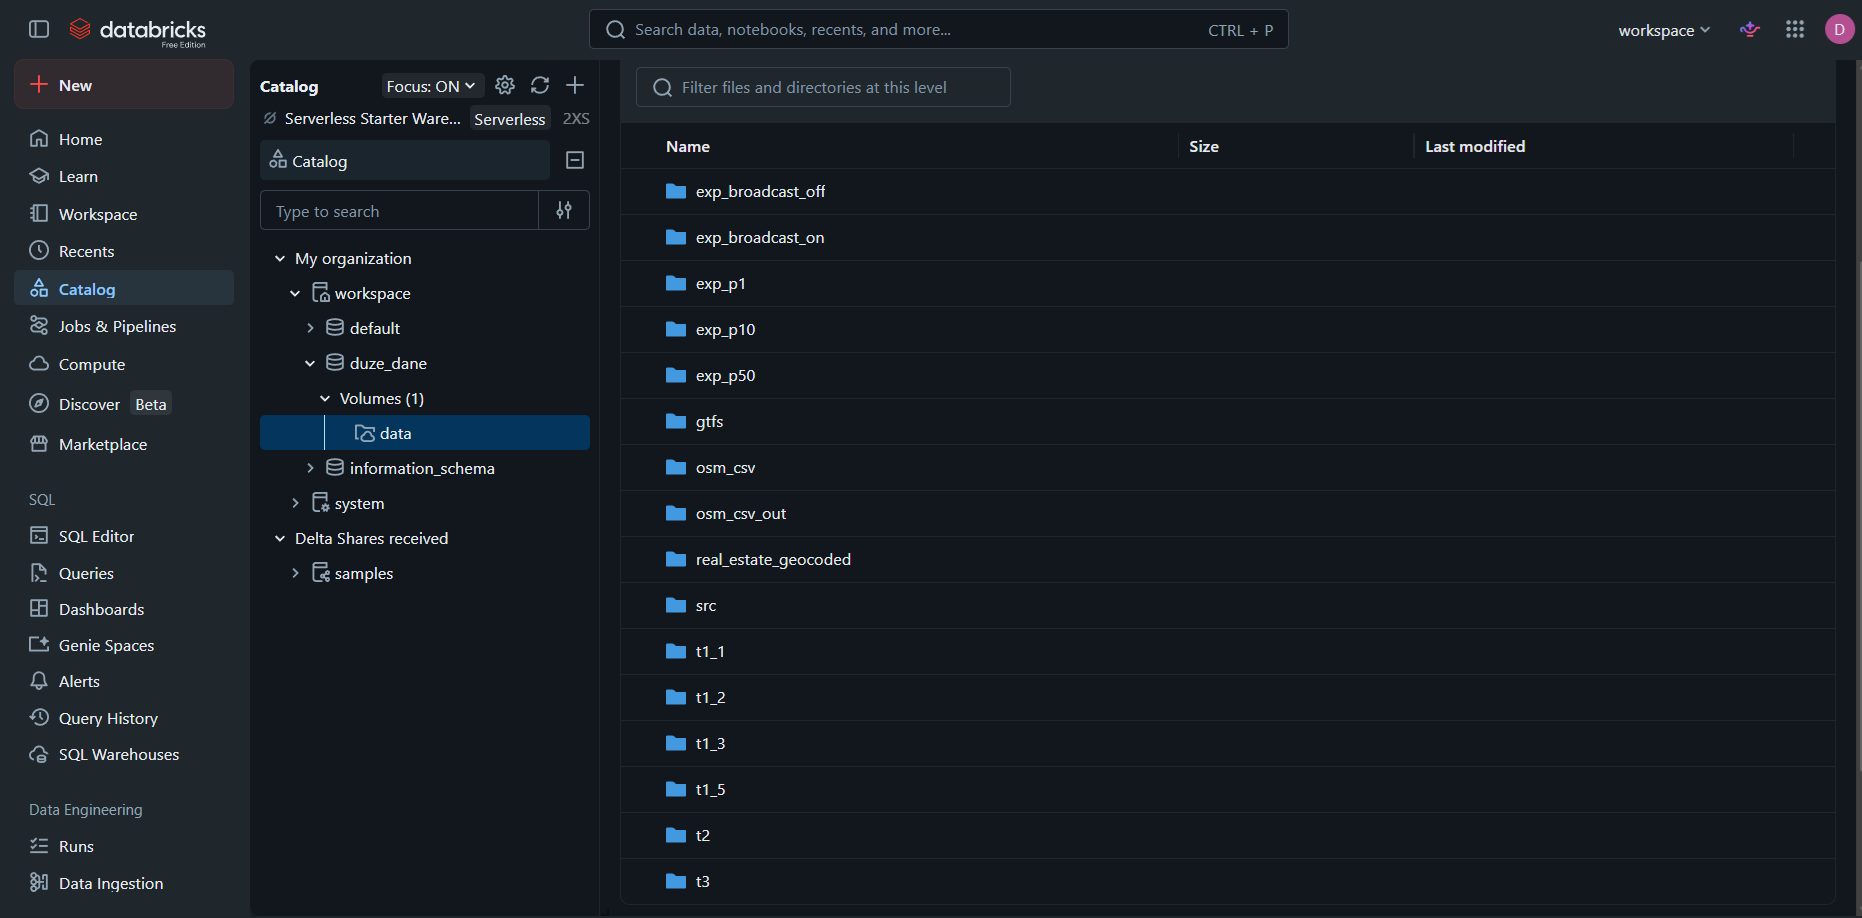
\includegraphics[width=0.95\textwidth]{img/catalog.png}
    \caption{Unity Catalog -- zawartość wolumenu \texttt{data} po wykonaniu potoku}
    \label{fig:catalog}
\end{figure}

\subsection{Workspace -- pliki źródłowe}

Skrypty PySpark wgrywane są do \textbf{Databricks Workspace} (nie do DBFS ani Volumes), ponieważ Databricks Free Edition nie obsługuje odczytu plików \texttt{.py} z~DBFS root w~trybie serverless. Rysunek~\ref{fig:workspace} pokazuje folder \texttt{/Workspace/duze-dane/src/} z~dwoma plikami: \texttt{spark\_pipeline.py} (główny potok) oraz \texttt{osm\_to\_csv.py} (konwersja danych OSM z~Parquet do CSV).

\begin{figure}[H]
    \centering
    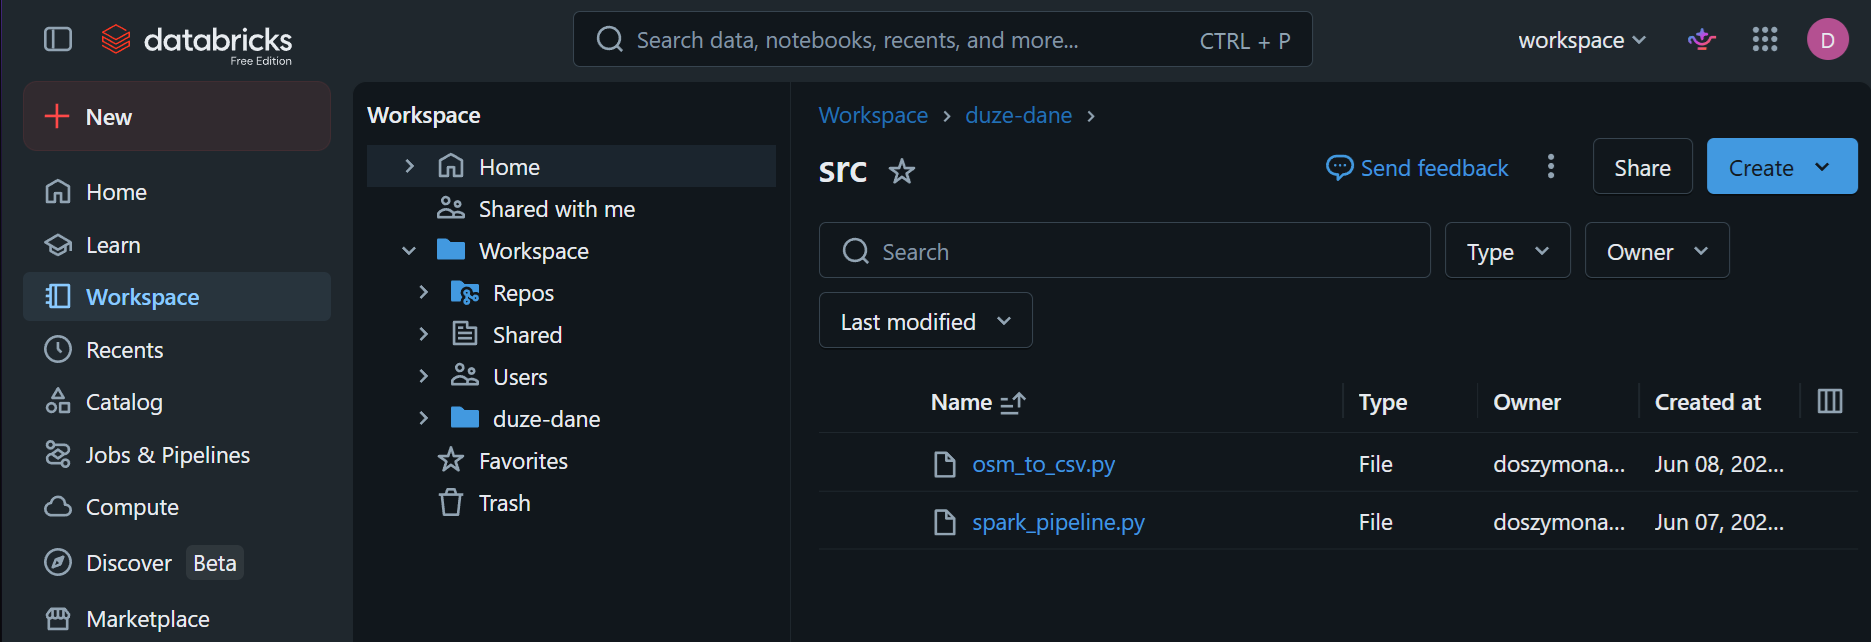
\includegraphics[width=0.95\textwidth]{img/workspace.png}
    \caption{Workspace Databricks -- pliki źródłowe potoku}
    \label{fig:workspace}
\end{figure}

\subsection{Wyniki w~wolumenie}

Rysunek~\ref{fig:success} przedstawia zawartość katalogu \texttt{t2} w~Unity Catalog -- wyniki etapu E2 zapisane jako pliki tekstowe w~formacie \texttt{part-XXXXX}. Plik \texttt{\_SUCCESS} sygnalizuje pomyślne zakończenie zapisu przez Spark.

\begin{figure}[H]
    \centering
    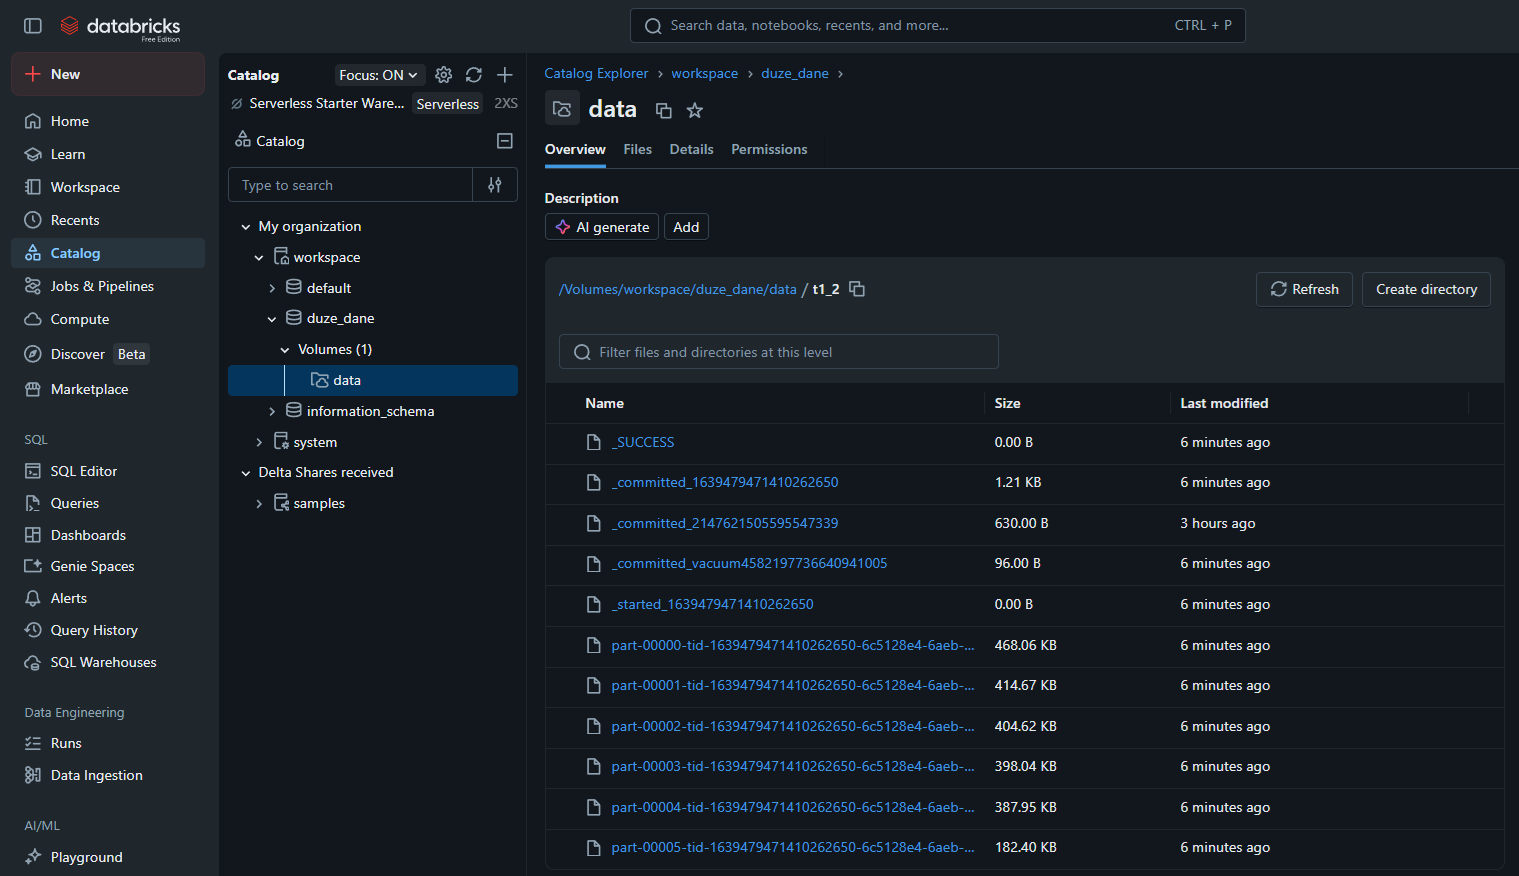
\includegraphics[width=0.95\textwidth]{img/success.png}
    \caption{Wyniki etapu E2 zapisane w~Unity Catalog Volume -- widoczne pliki \texttt{part-*} i~znacznik \texttt{\_SUCCESS}}
    \label{fig:success}
\end{figure}

\subsection{Ograniczenie Free Edition -- podział potoku na dwa joby}

Databricks Free Edition nakłada limit \textbf{5 równocześnie aktywnych tasków} na job. Pierwotna wersja potoku definiowała jeden job z~7 taskami -- próba jego uruchomienia kończyła się błędem widocznym na rysunku~\ref{fig:error}: \textit{,,There are already 5 active runs (limit: 5)''}.

\begin{figure}[H]
    \centering
    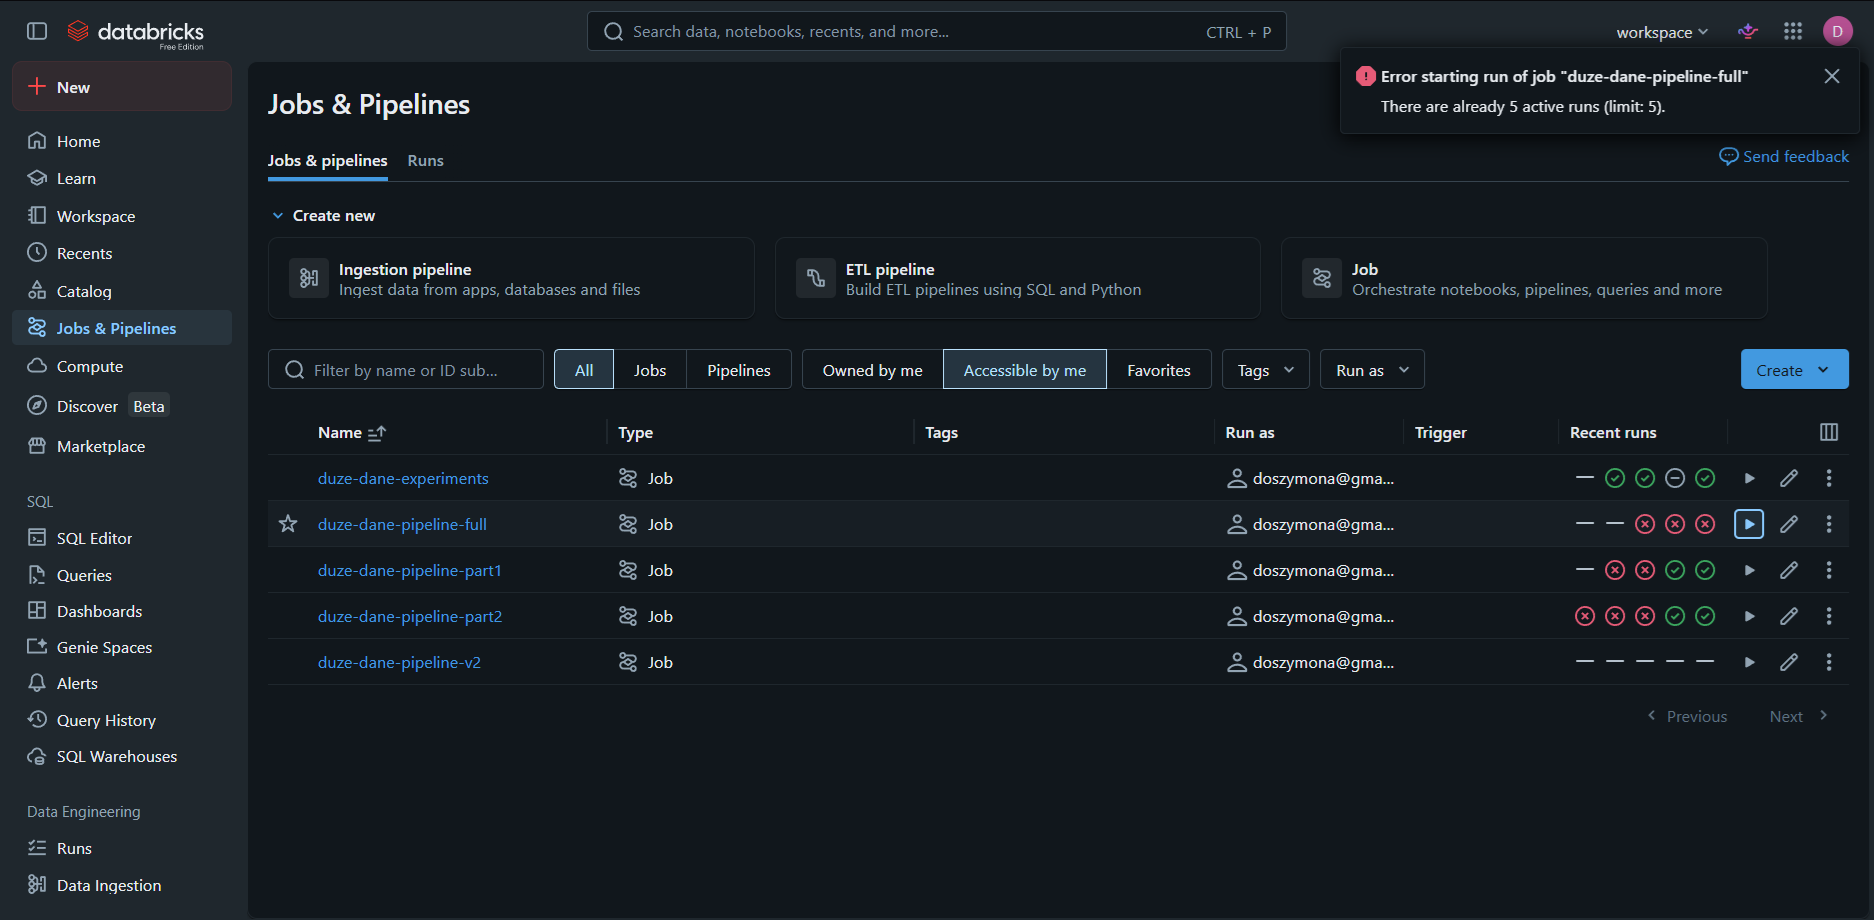
\includegraphics[width=0.95\textwidth]{img/error.png}
    \caption{Błąd uruchomienia joba z~więcej niż 5 taskami w~Databricks Free Edition}
    \label{fig:error}
\end{figure}

Z~tego powodu potok podzielono na dwa osobne joby:
\begin{itemize}
    \item \textbf{duze-dane-pipeline-part1} -- 5 tasków: \texttt{osm\_preprocess}, \texttt{e1\_1}, \texttt{e1\_5}, \texttt{e1\_2}, \texttt{e1\_3} (etapy przygotowania danych, uruchamiane równolegle tam gdzie brak zależności)
    \item \textbf{duze-dane-pipeline-part2} -- 2 taski: \texttt{e2} $\rightarrow$ \texttt{e3} (obliczenia wskaźników i~korelacji)
\end{itemize}

% ============================================================
\section{Implementacja potoku w~chmurze}
% ============================================================

\subsection{Adaptacje do środowiska serverless}

Wersja lokalna potoku (etap~9) korzystała z~RDD API oraz \texttt{sparkContext}, które są niedostępne w~Databricks serverless. Poniżej zestawiono wszystkie zmiany wprowadzone w~kodzie wraz z~uzasadnieniem.

\begin{description}
    \item[\textbf{E1.3 -- rzutowanie kolumn:}] Zamieniono \texttt{.cast("double")} na \texttt{expr("try\_cast(...) as double")}. Photon engine przerywa job błędem \texttt{CAST\_INVALID\_INPUT} gdy napotka nieprasowalną wartość; \texttt{try\_cast} zwraca \texttt{NULL} zamiast rzucać wyjątek.

    \item[\textbf{E2 -- logika obliczeń:}] Zastąpiono RDD (\texttt{.rdd.map()} $\rightarrow$ \texttt{groupByKey()} $\rightarrow$ \texttt{mapPartitions()}) przez DataFrame API (\texttt{union()} $\rightarrow$ \texttt{groupBy("geoId")} $\rightarrow$ \texttt{applyInPandas()}). Databricks serverless nie udostępnia \texttt{sparkContext}, który jest silnikiem RDD.

    \item[\textbf{E2 -- zapis wyników:}] Zamieniono \texttt{rdd.saveAsTextFile()} na \texttt{df.write.mode("overwrite").text()} -- z~tego samego powodu.

    \item[\textbf{E3 -- odczyt i~parsowanie:}] Zamieniono \texttt{sparkContext.textFile()} $\rightarrow$ \texttt{spark.read.text()} oraz \texttt{rdd.map().toDF()} $\rightarrow$ \texttt{mapInPandas()} -- z~tego samego powodu.

    \item[\textbf{E3 -- korelacja Pearsona:}] Zastąpiono Spark \texttt{corr(x, y)} w~\texttt{groupBy().agg()} przez pandas \texttt{.corr()} wywołane przez \texttt{groupBy().applyInPandas()}. Spark \texttt{corr()} rzuca \texttt{DIVIDE\_BY\_ZERO} gdy odchylenie standardowe kolumny wynosi~0 (wskaźniki są stałe w~obrębie geohasha); pandas zwraca w~takim przypadku \texttt{NaN}.

    \item[\textbf{osm\_to\_csv.py -- konfiguracja:}] Dodano \texttt{argparse} z~parametrami \texttt{--input}/\texttt{--output} zamiast hardcoded ścieżek HDFS. Konfiguracja YARN aktywna tylko gdy brak zmiennej środowiskowej \texttt{DATABRICKS\_RUNTIME\_VERSION}. Usunięto \texttt{spark\-Context.setLog\-Level()}, które jest niedostępne w~serverless.

    \item[\textbf{osm\_to\_csv.py -- odczyt danych:}] Zmieniono \texttt{spark.read.parquet(path)} na \texttt{spark.read.option("basePath",~path).parquet(path+"/parquet")}. Dane OSM w~Unity Catalog Volume przechowywane są w~podkatalogu \texttt{parquet/} jako partycjonowany Parquet -- bez jawnego podania \texttt{basePath} Spark nie potrafi scalić partycji.
\end{description}

\subsection{Przegląd etapów}

Potok przeniesiony do chmury realizuje te same etapy analityczne co wersja lokalna (etap~9), jednak z~szeregiem adaptacji wymaganych przez środowisko serverless Databricks:

\begin{itemize}
    \item \textbf{osm\_preprocess} -- konwersja danych OSM z~formatu GeoParquet (partycjonowane pliki w~\texttt{/osm\_csv/parquet/}) do CSV z~przypisaniem kategorii i~wag POI. Uruchamiany jako osobny task ze skryptu \texttt{osm\_to\_csv.py}.
    \item \textbf{E1.1} -- ekstrakcja i~normalizacja danych GTFS z~opcjonalnym broadcast join dla małych tabel referencyjnych. Wynik w~Parquet.
    \item \textbf{E1.5} -- pre-agregacja odjazdów GTFS w~godzinach szczytu (7--9), grupowanie per przystanek. Wynik w~Parquet.
    \item \textbf{E1.2} -- wczytanie znormalizowanego CSV z~POI, przypisanie klucza Geohash (precyzja~6). Wynik w~Parquet.
    \item \textbf{E1.3} -- normalizacja ofert nieruchomości: \texttt{try\_cast} zamiast \texttt{cast} (Photon engine nie toleruje błędów rzutowania), przypisanie Geohash. Wynik w~Parquet.
    \item \textbf{E2} -- scala trzy zbiory (przystanki, POI, oferty) po kluczu Geohash przez \texttt{applyInPandas} (RDD API niedostępne w~serverless). Dla każdej oferty oblicza wskaźniki Haversine w~promieniu 800~m.
    \item \textbf{E3} -- parsuje wyjście E2, grupuje per miasto przez \texttt{applyInPandas} i~oblicza korelacje Pearsona w~pandas (Spark \texttt{corr()} rzuca \texttt{DIVIDE\_BY\_ZERO} przy zerowej wariancji).
\end{itemize}

\subsection{Grafy wykonania jobów}

Rysunek~\ref{fig:part1} przedstawia graf DAG joba \texttt{pipeline-part1}. Taski \texttt{osm\_preprocess}, \texttt{e1\_1} i~\texttt{e1\_3} uruchamiane są równolegle. Po zakończeniu \texttt{e1\_1} startuje \texttt{e1\_5}, a~po \texttt{osm\_preprocess} -- \texttt{e1\_2}.

\begin{figure}[H]
    \centering
    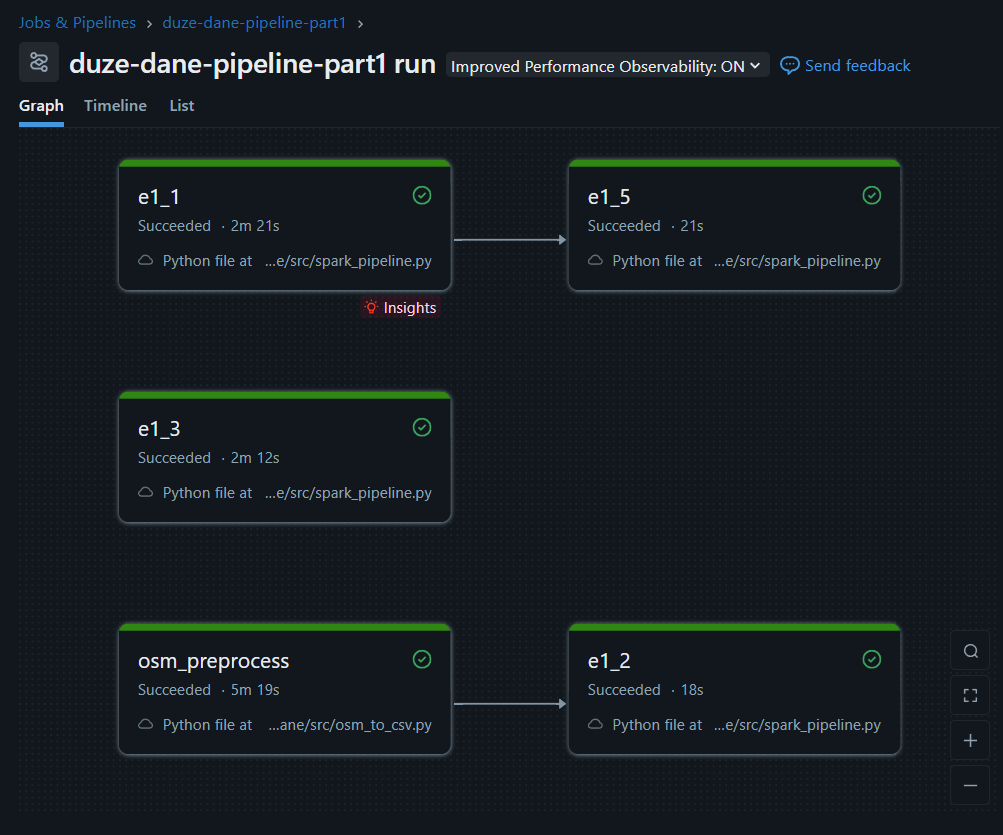
\includegraphics[width=0.85\textwidth]{img/pipeline-part1.png}
    \caption{Graf wykonania joba \texttt{duze-dane-pipeline-part1}}
    \label{fig:part1}
\end{figure}

\begin{figure}[H]
    \centering
    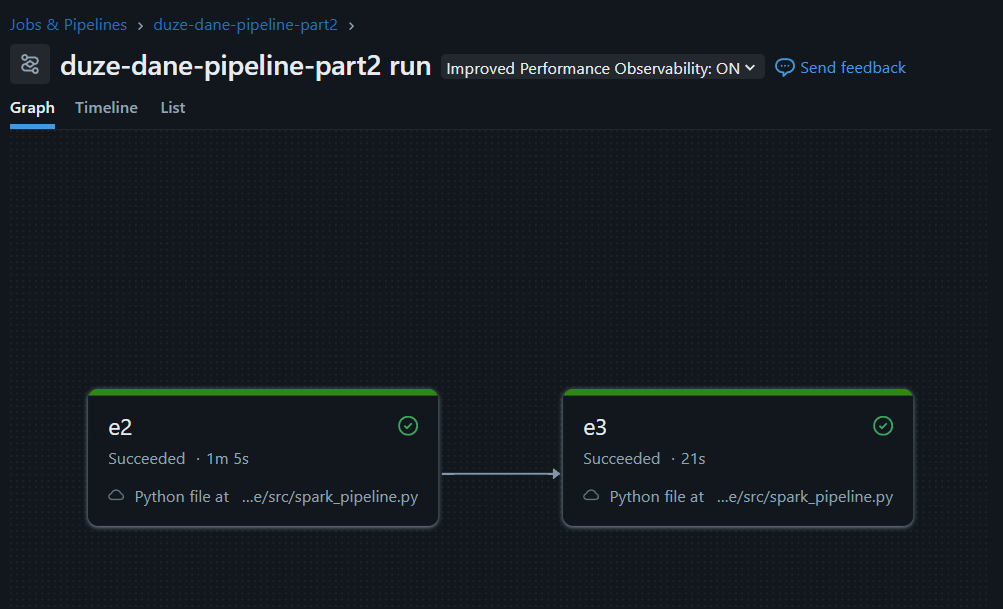
\includegraphics[width=0.75\textwidth]{img/pipeline-part2.png}
    \caption{Graf wykonania joba \texttt{duze-dane-pipeline-part2}}
    \label{fig:part2}
\end{figure}

% ============================================================
\section{Czasy wykonania potoku w~chmurze}
% ============================================================

\begin{table}[H]
\centering
\caption{Czasy wykonania poszczególnych etapów potoku w~Databricks serverless}
\label{tab:cloud_times}
\renewcommand{\arraystretch}{1.3}
\begin{tabular}{|l|p{6cm}|c|}
\hline
\rowcolor{gray!20}
\textbf{Task} & \textbf{Opis} & \textbf{Czas [s]} \\ \hline
\textbf{osm\_preprocess} & Konwersja OSM Parquet $\rightarrow$ CSV & 319 \\ \hline
\textbf{E1.1}            & Ekstrakcja GTFS + broadcast join       & 141 \\ \hline
\textbf{E1.5}            & Agregacja GTFS (odjazdy/przystanek)    & 21  \\ \hline
\textbf{E1.2}            & Ekstrakcja POI z~OSM                   & 18  \\ \hline
\textbf{E1.3}            & Normalizacja ofert nieruchomości       & 132 \\ \hline
\textbf{E2}              & Wskaźniki per oferta (applyInPandas)   & 65  \\ \hline
\textbf{E3}              & Korelacja Pearsona per miasto          & 21  \\ \hline
\rowcolor{gray!10}
\multicolumn{2}{|r|}{\textbf{Part 1 (równolegle)}} & \textbf{~360} \\ \hline
\rowcolor{gray!10}
\multicolumn{2}{|r|}{\textbf{Part 2}} & \textbf{153} \\ \hline
\end{tabular}
\end{table}

Taski w~Part~1 uruchamiane są częściowo równolegle (rysunek~\ref{fig:part1-timeline}), przez co czas całkowity wynosi około 360~s, a~nie sumę wszystkich etapów.

\begin{figure}[H]
    \centering
    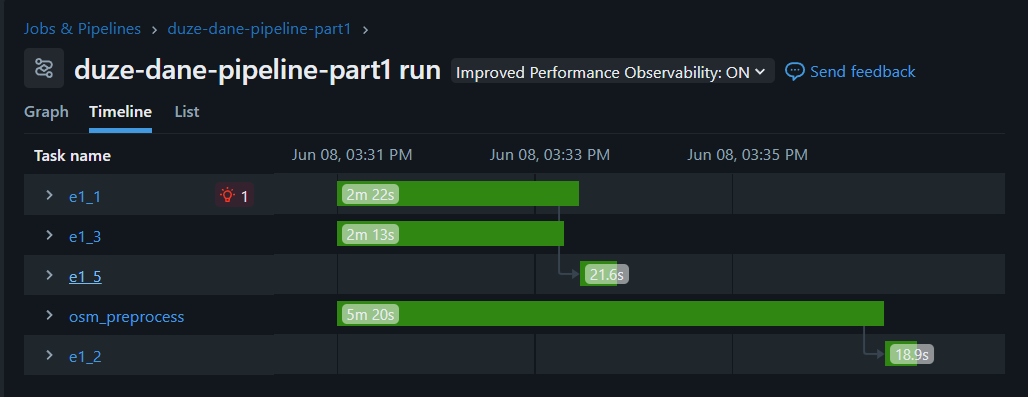
\includegraphics[width=0.95\textwidth]{img/pipeline-part1-timeline.png}
    \caption{Timeline wykonania joba \texttt{duze-dane-pipeline-part1} -- widoczne równoległe uruchomienie tasków}
    \label{fig:part1-timeline}
\end{figure}

\begin{figure}[H]
    \centering
    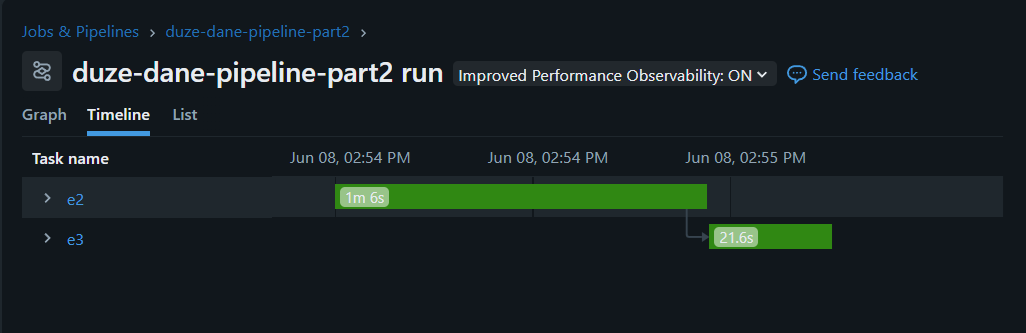
\includegraphics[width=0.95\textwidth]{img/pipeline-part2-timeline.png}
    \caption{Timeline wykonania joba \texttt{duze-dane-pipeline-part2}}
    \label{fig:part2-timeline}
\end{figure}

\subsection{Porównanie: chmura vs.\ on-premise}

\begin{table}[H]
\centering
\caption{Porównanie czasów wykonania etapów Spark on-premise vs.\ Databricks serverless}
\label{tab:comparison}
\renewcommand{\arraystretch}{1.3}
\begin{tabular}{|l|c|c|c|}
\hline
\rowcolor{gray!20}
\textbf{Etap} & \textbf{On-premise [s]} & \textbf{Databricks [s]} & \textbf{Różnica} \\ \hline
E1.1 & 24  & 141 & $\times$5.9 wolniej \\ \hline
E1.5 & 17  & 21  & $\times$1.2 wolniej \\ \hline
E1.2 & 17  & 18  & $\approx$ tyle samo \\ \hline
E1.3 & 21  & 132 & $\times$6.3 wolniej \\ \hline
E2   & 26  & 65  & $\times$2.5 wolniej \\ \hline
E3   & 19  & 21  & $\approx$ tyle samo \\ \hline
\rowcolor{gray!10}
\textbf{Łącznie (sekwencyjnie)} & \textbf{124} & \textbf{717} & $\times$5.8 wolniej \\ \hline
\end{tabular}
\end{table}

Databricks serverless okazuje się wolniejszy od lokalnego klastra Spark dla większości etapów. Główne przyczyny:
\begin{itemize}
    \item \textbf{Python UDF overhead} -- etapy E1.1 i~E1.3 intensywnie używają UDF (geohash), który w~serverless uruchamiany jest przez \texttt{Batch Eval Python} bez możliwości JIT. Na lokalnym klastrze ten sam UDF korzystał z~zoptymalizowanego środowiska executora.
    \item \textbf{Cold start serverless} -- każdy task czeka na przydzielenie zasobów (widoczne w~timeline jako przerwa przed faktycznym wykonaniem).
    \item \textbf{applyInPandas zamiast RDD} -- etap E2 wymaga transferu danych do procesu Python per grupę Geohash, co jest wolniejsze niż natywne RDD na lokalnym klastrze.
    \item \textbf{E1.2 i~E3} -- etapy o~prostej logice (scan + aggregate, scan + mapInPandas) nie różnią się istotnie, ponieważ dominuje czas I/O, nie obliczenia.
\end{itemize}

% ============================================================
\section{Eksperymenty}
% ============================================================

\subsection{Eksperyment A: Broadcast Join vs.\ Sort-Merge Join (E1.1)}

Eksperyment ten powielono w~chmurze. Wyniki przedstawia rysunek~\ref{fig:experiments} oraz tabela~\ref{tab:broadcast}.

\begin{figure}[H]
    \centering
    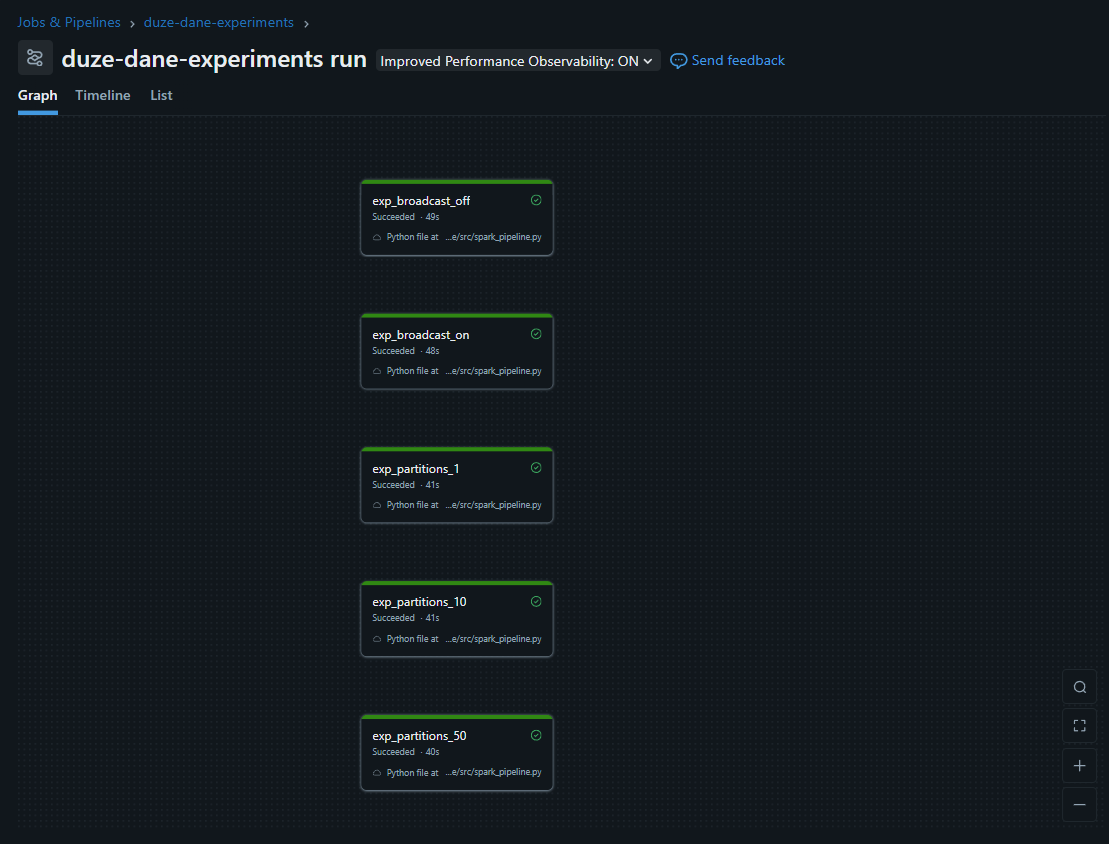
\includegraphics[width=0.85\textwidth]{img/experiments.png}
    \caption{Graf wykonania joba \texttt{duze-dane-experiments} -- eksperymenty broadcast i~partycje}
    \label{fig:experiments}
\end{figure}

\begin{figure}[H]
    \centering
    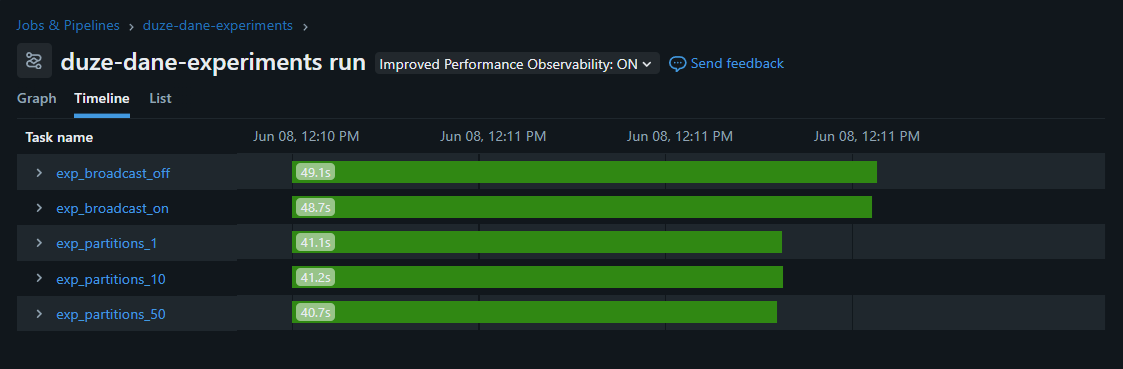
\includegraphics[width=0.95\textwidth]{img/experiments-timeline.png}
    \caption{Timeline joba \texttt{duze-dane-experiments} -- wszystkie taski uruchamiane równolegle}
    \label{fig:experiments-timeline}
\end{figure}

\begin{table}[H]
\centering
\caption{Wyniki eksperymentu A -- Broadcast Join vs.\ Sort-Merge Join (E1.1) w~chmurze}
\label{tab:broadcast}
\renewcommand{\arraystretch}{1.3}
\begin{tabular}{|l|c|}
\hline
\rowcolor{gray!20}
\textbf{Wariant} & \textbf{Czas [s]} \\ \hline
Broadcast włączony  & 48 \\ \hline
Broadcast wyłączony & 49 \\ \hline
\end{tabular}
\end{table}

\textbf{Wniosek:} W~środowisku serverless różnica między broadcast join a~sort-merge join jest minimalna (1~s). Photon engine oraz Catalyst Optimizer samodzielnie decydują o~strategii złączenia, a~wolumen danych GTFS jest wystarczająco mały, by różnica strategii była niezauważalna.

\subsection{Eksperyment B: Liczba partycji shuffle (E1.5)}

\begin{table}[H]
\centering
\caption{Wyniki eksperymentu B -- liczba partycji shuffle w~E1.5 w~chmurze}
\label{tab:partitions}
\renewcommand{\arraystretch}{1.3}
\begin{tabular}{|c|c|}
\hline
\rowcolor{gray!20}
\textbf{Liczba partycji} & \textbf{Czas [s]} \\ \hline
1  & 41 \\ \hline
10 & 41 \\ \hline
50 & 40 \\ \hline
\end{tabular}
\end{table}

\textbf{Wniosek:} W~środowisku serverless parametr \texttt{spark.sql.shuffle.partitions} praktycznie nie wpływa na czas wykonania. Photon engine zarządza partycjonowaniem adaptywnie (Adaptive Query Execution), ignorując ustawienie ręczne. Na lokalnym klastrze przy 1~partycji uzyskano 14.7~s vs.\ 18.0~s dla 50 partycji -- różnica była wyraźna. W~chmurze AQE niweluje ten efekt.

\subsection{Eksperyment C: DataFrame API vs.\ Spark SQL (E1.5)}

Dodatkowy eksperyment przeprowadzony wyłącznie w~chmurze porównuje implementację E1.5 przez natywne DataFrame API PySpark z~wersją opartą na Spark SQL. Poniżej przedstawiono oba warianty implementacji:

\begin{minted}{python}
# Wariant DataFrame API
def run_e1_5(spark, input_path, output_path, reducers=1):
    df = spark.read.parquet(input_path)
    df = df.withColumn("hour", split(col("arrival_time"), ":")[0].cast("int"))
    df = df.filter((col("hour") >= 7) & (col("hour") <= 9))
    agg_df = df.groupBy("stop_id", "stop_lat", "stop_lon", "geoId") \
               .count().withColumnRenamed("count", "score")
    agg_df.write.parquet(output_path, mode="overwrite")

# Wariant Spark SQL
def run_e1_5_sql(spark, input_path, output_path, reducers=1):
    df = spark.read.parquet(input_path)
    df.createOrReplaceTempView("stop_times_raw")
    agg_df = spark.sql("""
        SELECT stop_id, stop_lat, stop_lon, geoId, COUNT(*) AS score
        FROM stop_times_raw
        WHERE CAST(SPLIT(arrival_time, ':')[0] AS INT) BETWEEN 7 AND 9
        GROUP BY stop_id, stop_lat, stop_lon, geoId
    """)
    agg_df.write.parquet(output_path, mode="overwrite")
\end{minted}

\begin{figure}[H]
    \centering
    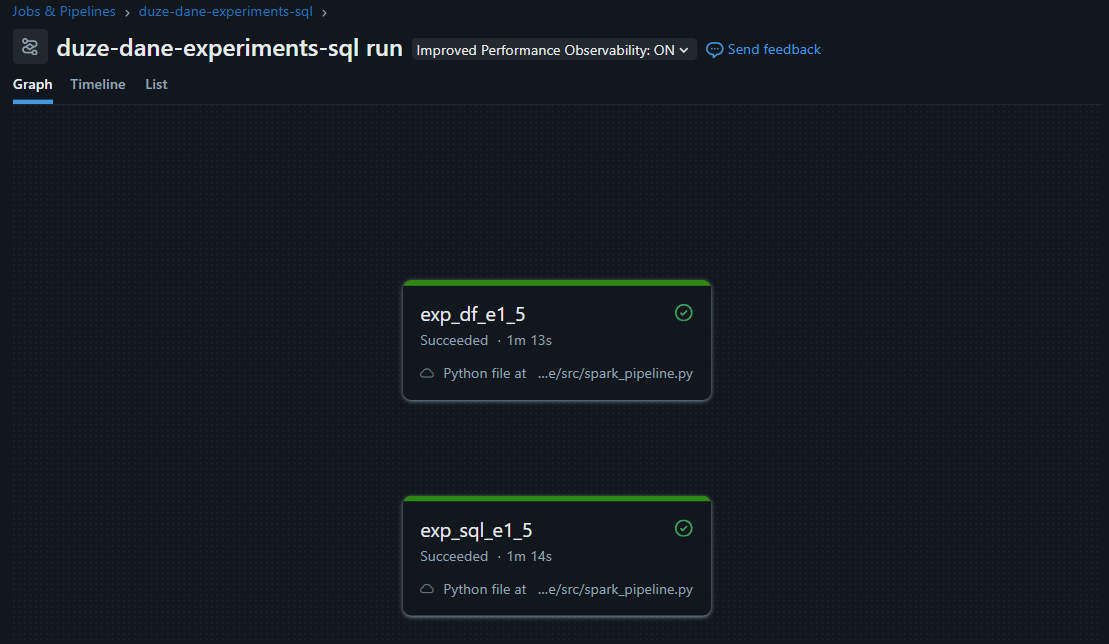
\includegraphics[width=0.75\textwidth]{img/experiments-sql.png}
    \caption{Graf wykonania joba \texttt{duze-dane-experiments-sql} -- DataFrame API vs.\ Spark SQL}
    \label{fig:experiments-sql}
\end{figure}

\begin{table}[H]
\centering
\caption{Wyniki eksperymentu C -- DataFrame API vs.\ Spark SQL w~E1.5}
\label{tab:sql}
\renewcommand{\arraystretch}{1.3}
\begin{tabular}{|l|c|}
\hline
\rowcolor{gray!20}
\textbf{Wariant} & \textbf{Czas [s]} \\ \hline
DataFrame API & 73 \\ \hline
Spark SQL     & 74 \\ \hline
\end{tabular}
\end{table}

\textbf{Wniosek:} Oba warianty uzyskały identyczny czas wykonania. Potwierdza to, że Spark SQL jest jedynie warstwą składniową nad DataFrame API -- Catalyst Optimizer kompiluje oba zapisy do tego samego planu fizycznego. Potwierdzają to również query profile (rysunki~\ref{fig:qp-df} i~\ref{fig:qp-sql}), które pokazują identyczną sekwencję operatorów: \texttt{Scan} $\rightarrow$ \texttt{Grouping Aggregate} $\rightarrow$ \texttt{Shuffle} $\rightarrow$ \texttt{Grouping Aggregate} $\rightarrow$ \texttt{Write Into}.

\begin{figure}[H]
    \centering
    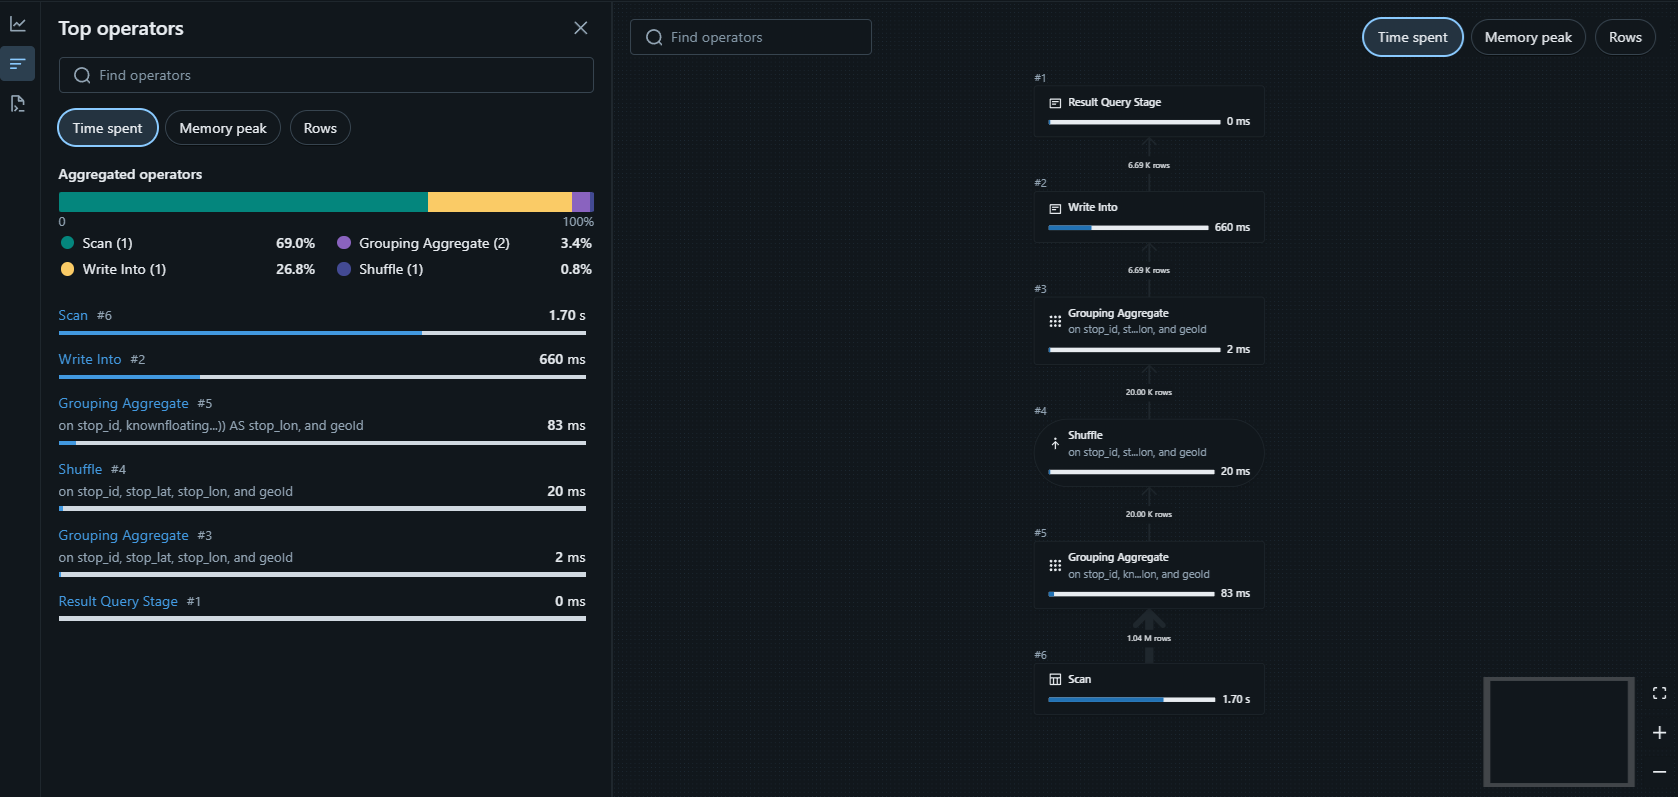
\includegraphics[width=0.95\textwidth]{img/qp-exp-df-e1-5.png}
    \caption{Query Profile dla E1.5 -- DataFrame API: Scan 1.70s, Write Into 660ms, Grouping Aggregate 83ms}
    \label{fig:qp-df}
\end{figure}

\begin{figure}[H]
    \centering
    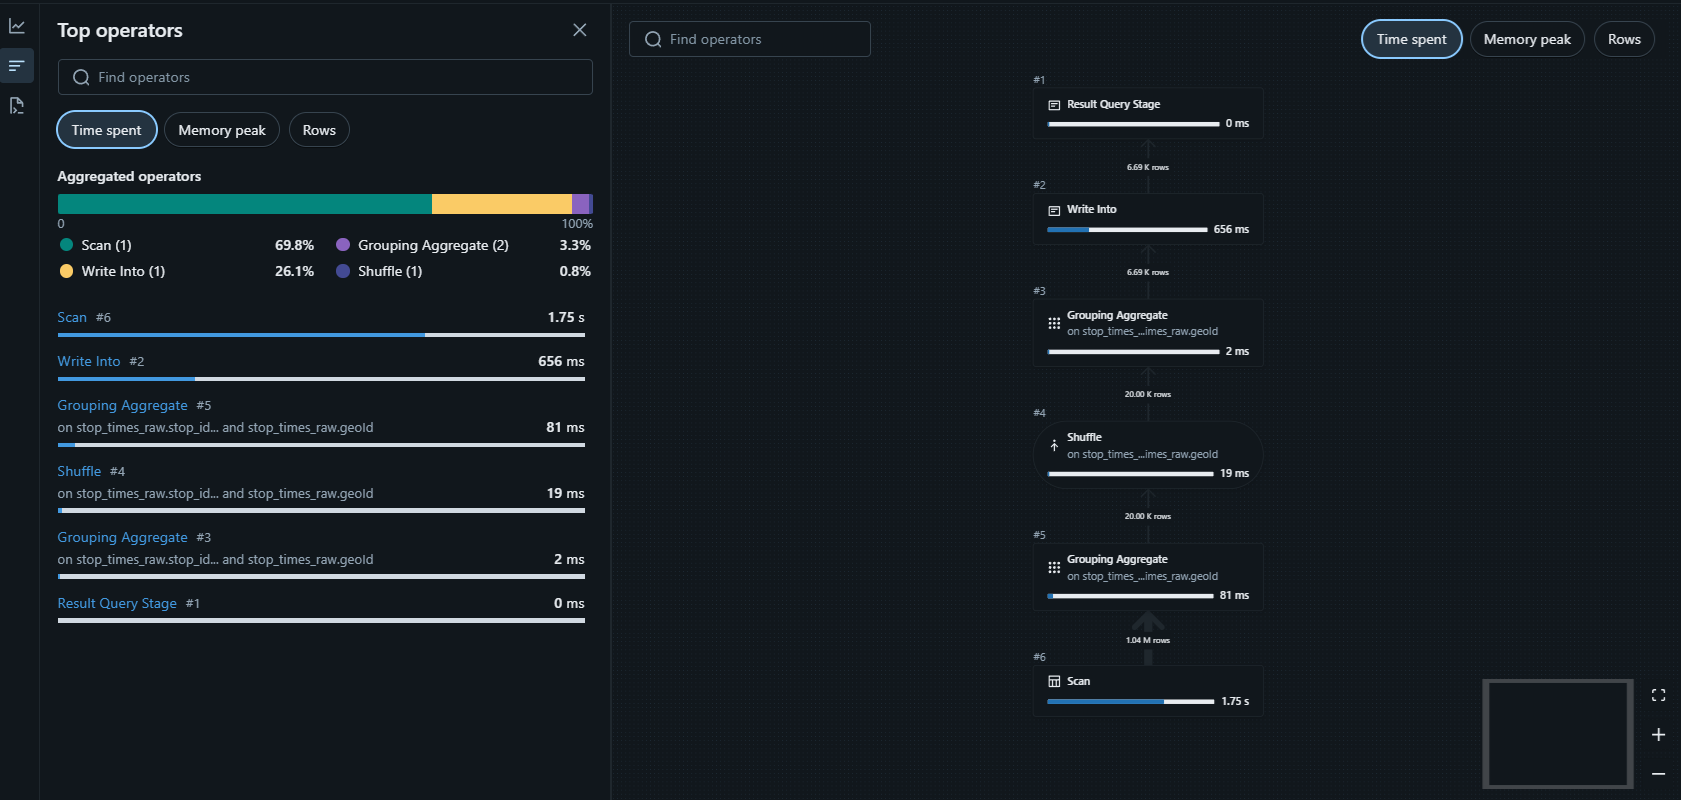
\includegraphics[width=0.95\textwidth]{img/qp-exp-sql-e1-5.png}
    \caption{Query Profile dla E1.5 -- Spark SQL: Scan 1.75s, Write Into 656ms, Grouping Aggregate 81ms}
    \label{fig:qp-sql}
\end{figure}

% ============================================================
\section{Query Profile -- analiza planów wykonania}
% ============================================================

Dla każdego etapu potoku zebrano Query Profile z~Databricks serverless. Profile przedstawiają fizyczny plan wykonania z~czasami poszczególnych operatorów.

\subsection{E1.1 -- Ekstrakcja GTFS}

\begin{figure}[H]
    \centering
    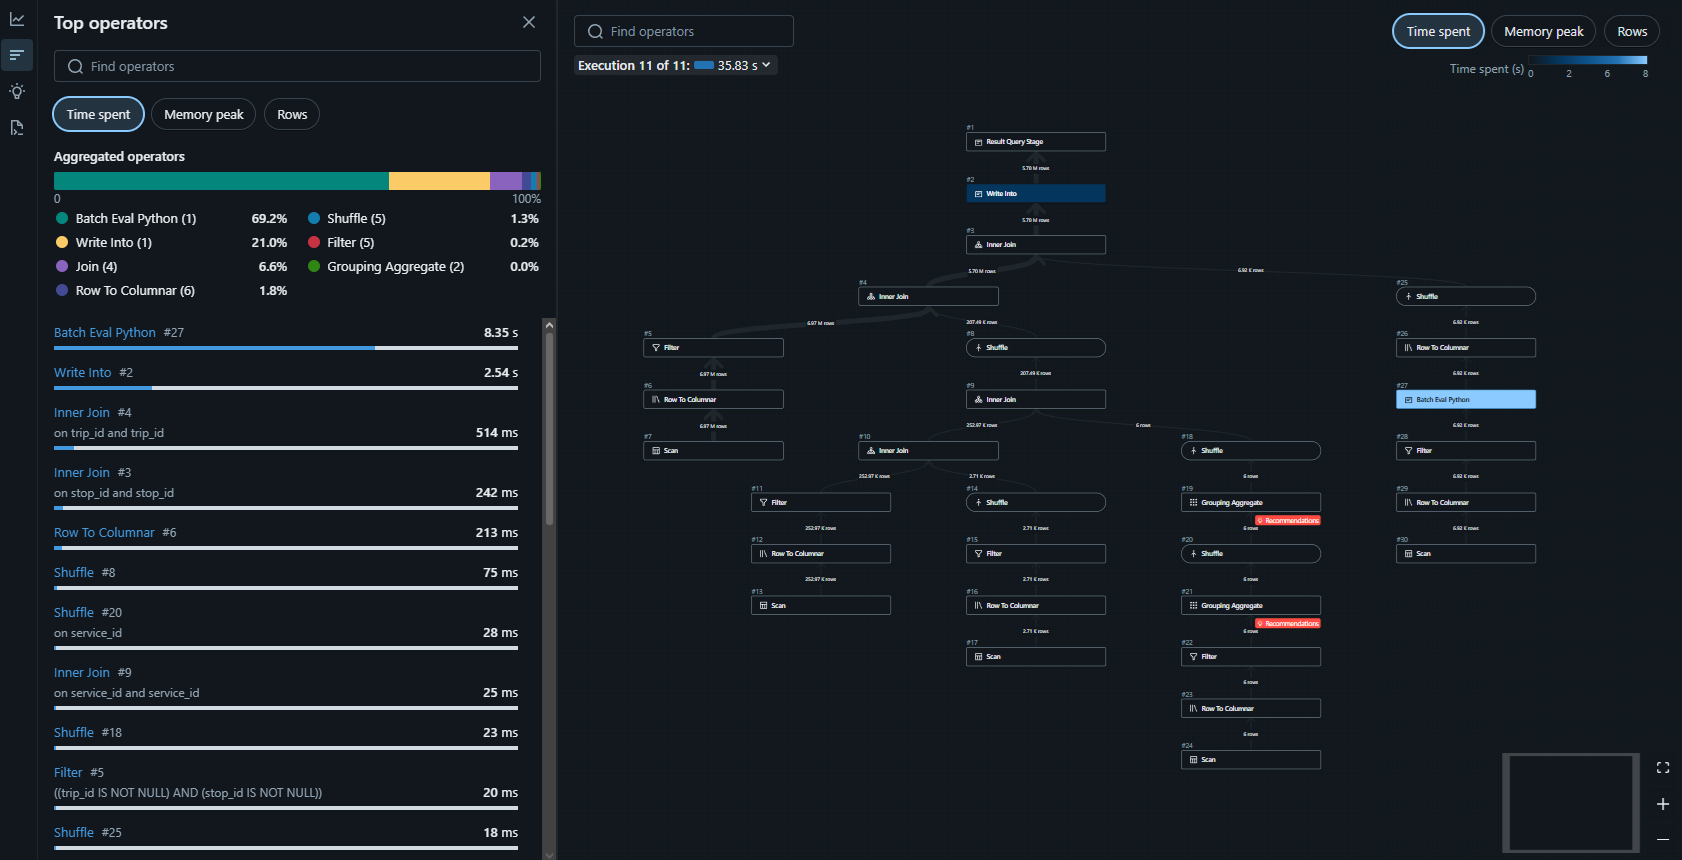
\includegraphics[width=0.95\textwidth]{img/qp-e1_1.png}
    \caption{Query Profile E1.1: dominuje \texttt{Batch Eval Python} (8.35s, 69\%) -- UDF geohasha. Widoczne 4 złączenia \texttt{Inner Join} i~5 operacji \texttt{Shuffle}.}
    \label{fig:qp-e1_1}
\end{figure}

Plan zawiera 4 złączenia \texttt{Inner Join} (po \texttt{trip\_id}, \texttt{stop\_id}, \texttt{service\_id}, \texttt{route\_id}), 5 operacji Shuffle oraz \texttt{Batch Eval Python} dla UDF geohasha. Operator \texttt{Batch Eval Python} zajmuje 69\% całkowitego czasu -- jest to główne wąskie gardło etapu E1.1 w~chmurze.

\subsection{E1.5 -- Agregacja GTFS}

\begin{figure}[H]
    \centering
    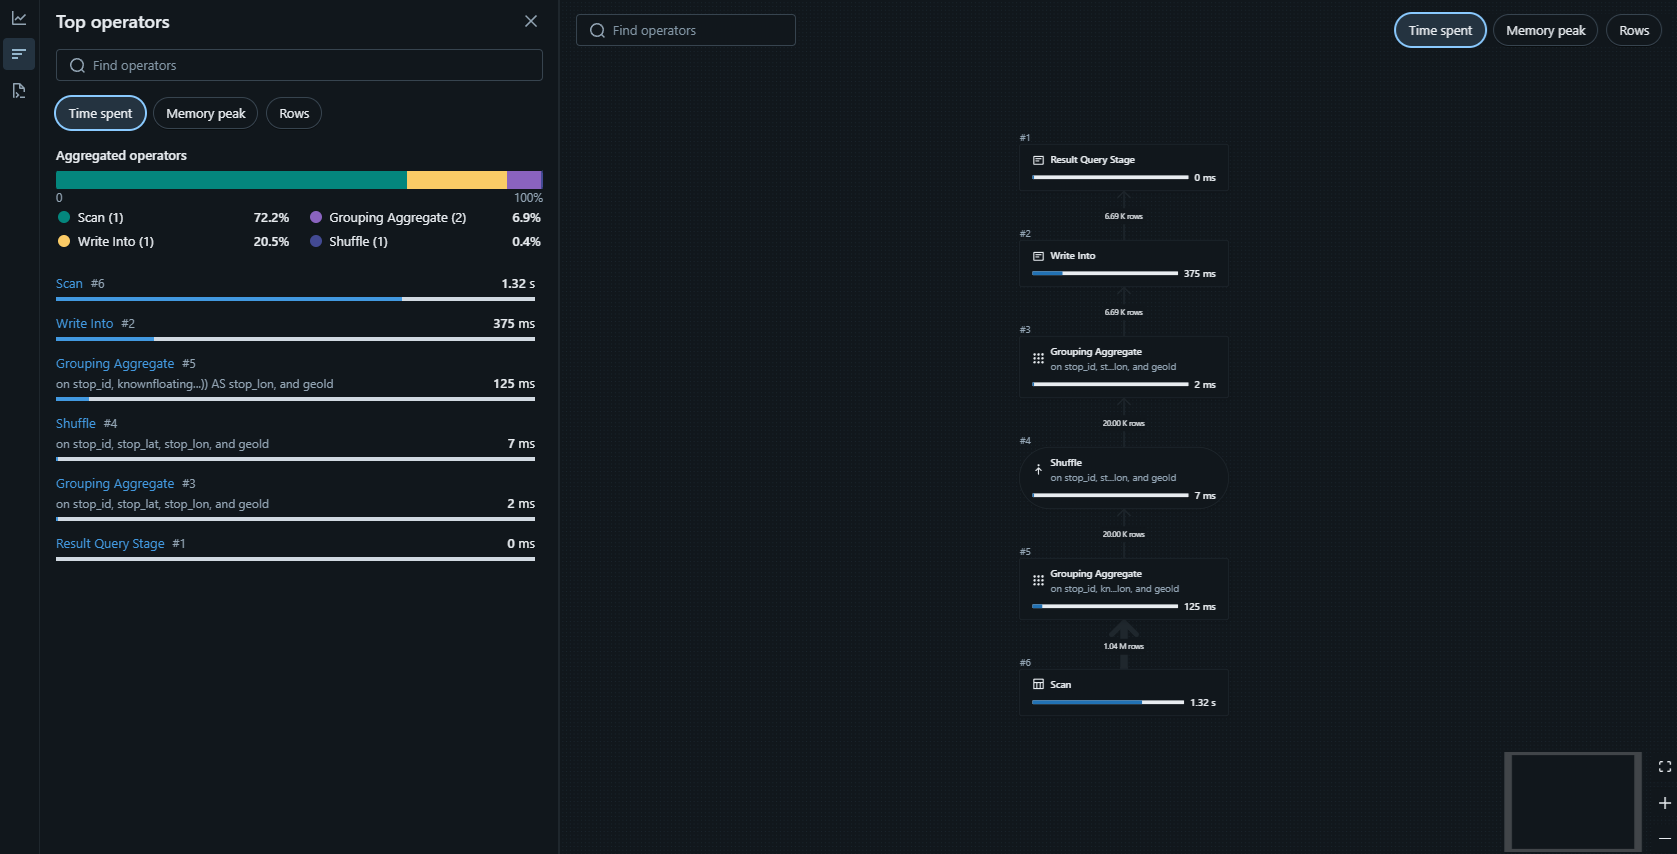
\includegraphics[width=0.95\textwidth]{img/qp-e1_5.png}
    \caption{Query Profile E1.5: prosty plan -- Scan (1.32s, 72\%) $\rightarrow$ dwustopniowa agregacja $\rightarrow$ Write Into (375ms).}
    \label{fig:qp-e1_5}
\end{figure}

Etap E1.5 ma najprostszy plan spośród wszystkich: wczytanie danych Parquet (Scan), dwustopniowa agregacja z~Shuffle pomiędzy (partial aggregate $\rightarrow$ shuffle $\rightarrow$ final aggregate), zapis wyników. Dominuje czas odczytu danych (72\%).

\subsection{E1.3 -- Normalizacja nieruchomości}

\begin{figure}[H]
    \centering
    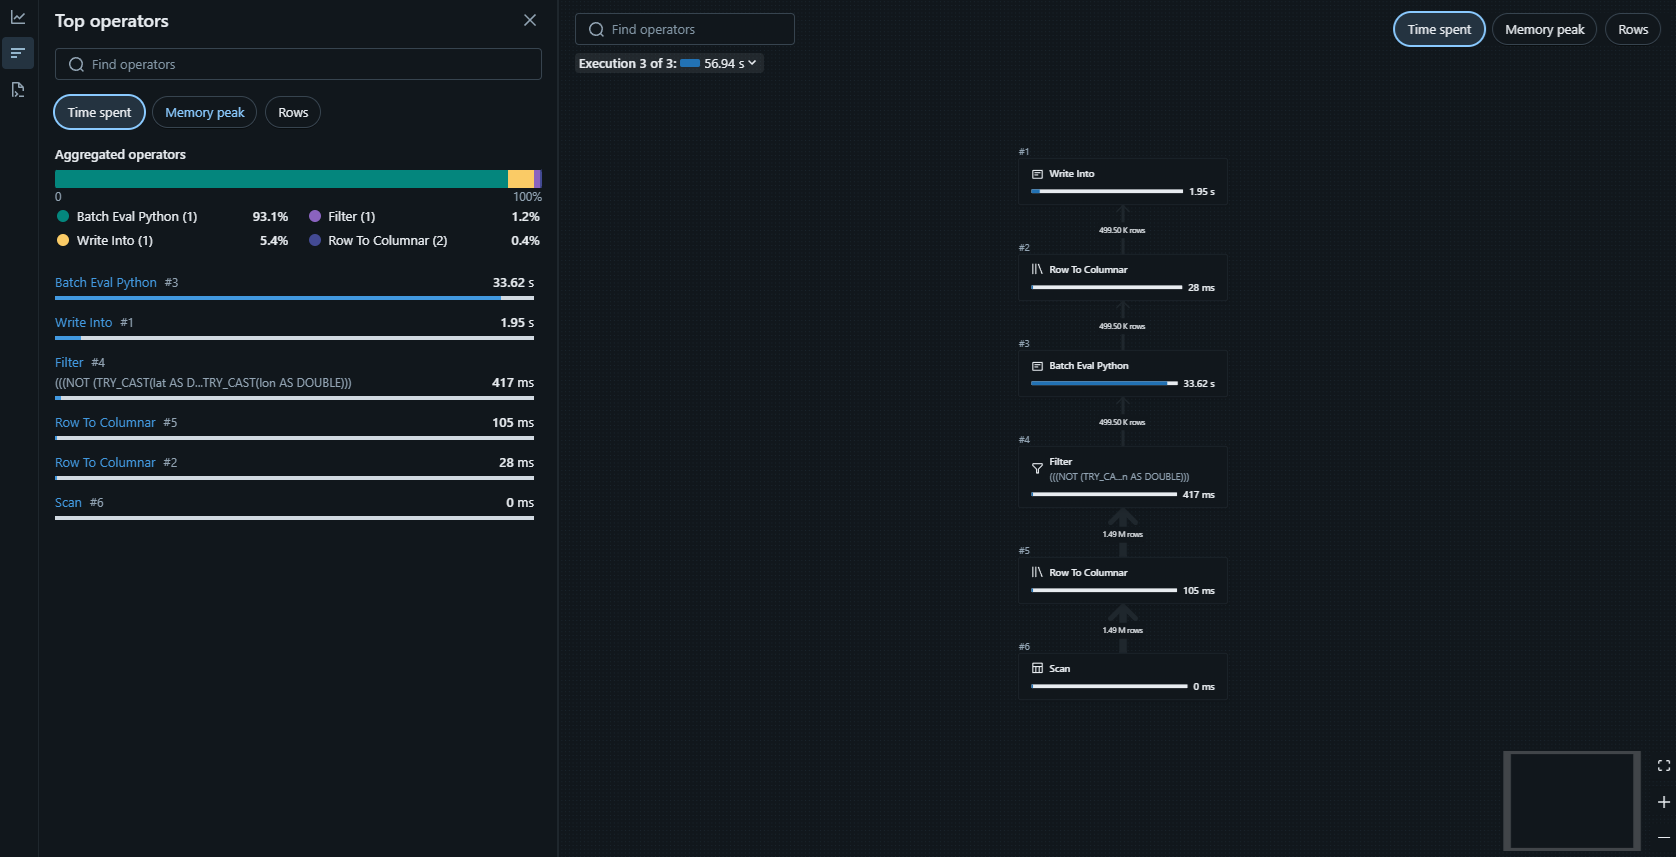
\includegraphics[width=0.95\textwidth]{img/qp-e1_3.png}
    \caption{Query Profile E1.3: \texttt{Batch Eval Python} (33.62s, 93\%) -- UDF geohasha na 1.49M rekordach nieruchomości.}
    \label{fig:qp-e1_3}
\end{figure}

Podobnie jak E1.1, etap E1.3 zdominowany jest przez \texttt{Batch Eval Python} (93\% czasu). Zbiór nieruchomości liczy 1.49M rekordów, co przy obliczaniu Geohasha przez Python UDF generuje znaczący overhead. Widoczny jest również operator \texttt{Filter} dla predykatu \texttt{TRY\_CAST(lat AS DOUBLE)}.

\subsection{E2 -- Obliczanie wskaźników}

\begin{figure}[H]
    \centering
    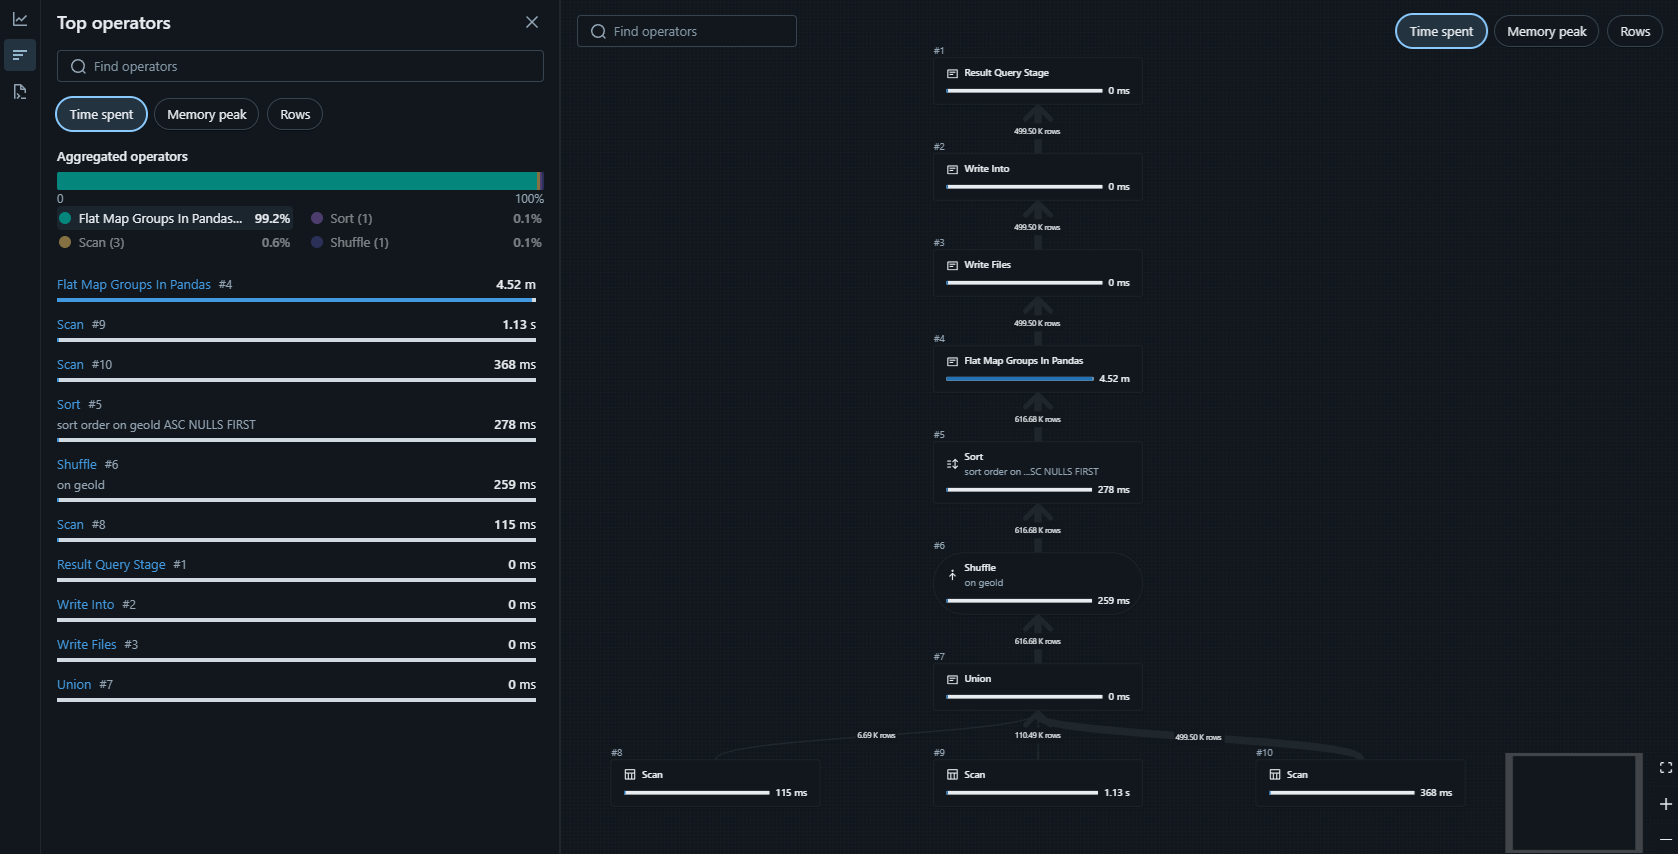
\includegraphics[width=0.95\textwidth]{img/qp_e2.png}
    \caption{Query Profile E2: \texttt{Flat Map Groups In Pandas} (4.52 min, 99.2\%) -- logika Haversine przez \texttt{applyInPandas}. Shuffle po \texttt{geoId} 259ms.}
    \label{fig:qp-e2}
\end{figure}

Etap E2 jest najbardziej czasochłonny -- operator \texttt{Flat Map Groups In Pandas} (odpowiednik \texttt{applyInPandas}) zajmuje 99.2\% czasu. Poprzedza go \texttt{Shuffle} po kluczu \texttt{geoId} (259ms), który grupuje dane przed przekazaniem do funkcji Python. Trzy \texttt{Scan} odpowiadają wczytaniu t1\_5, t1\_2 i~t1\_3, \texttt{Union} scala te zbiory przed shuffle.

\subsection{E3 -- Korelacja Pearsona}

\begin{figure}[H]
    \centering
    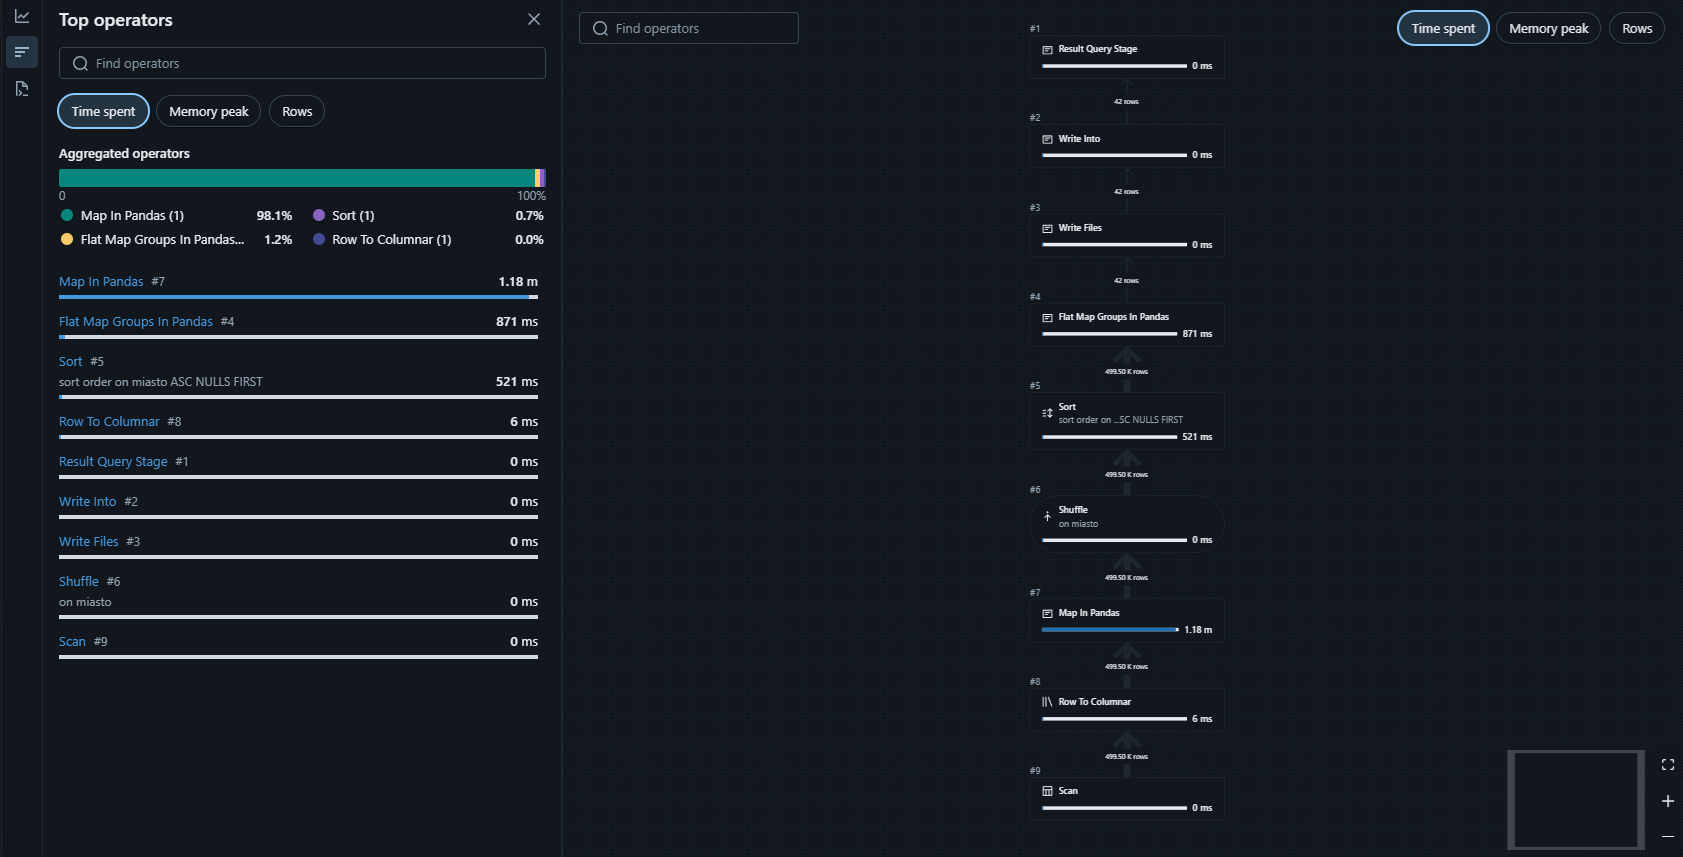
\includegraphics[width=0.95\textwidth]{img/qp-e3.png}
    \caption{Query Profile E3: \texttt{Map In Pandas} (dominuje) -- korelacje Pearsona obliczane przez pandas per miasto.}
    \label{fig:qp-e3}
\end{figure}

Etap E3 używa \texttt{applyInPandas} per miasto do obliczenia korelacji Pearsona. Spark SQL \texttt{corr()} został zastąpiony przez pandas \texttt{.corr()}, ponieważ wbudowana funkcja Sparka rzuca wyjątek \texttt{DIVIDE\_BY\_ZERO} gdy odchylenie standardowe kolumny wynosi 0 (wskaźniki identyczne w~obrębie geohasha). Pandas zwraca w~takim przypadku \texttt{NaN}, który zamieniany jest na 0.0.

\end{document}
